%% LyX 2.1.4 created this file.  For more info, see http://www.lyx.org/.
%% Do not edit unless you really know what you are doing.
\documentclass[english]{article}
\usepackage[T1]{fontenc}
\usepackage[latin9]{inputenc}
\usepackage{amstext}
\usepackage{graphicx}
\usepackage{babel}
\begin{document}

\title{Gravitino Lifetime and Neutrino Masses in Trilinear RpV}

\maketitle

\section{Gravitino Lifetime}

The full expressions for the gravitino decay width, considering trilinear
R-Parity violation, are given in hep-ph/017286. For instance, from
these expressions we can get an approximated formula for the leptonic
decay $\Gamma(\tilde{G}\rightarrow\nu_{i}e_{j}\bar{e}_{k})$ by assuming
that the mass of the sleptons that mediate the three body decay are
equal, such that $m_{\tilde{\nu}_{iL}}=m_{\tilde{e}_{jL}}=m_{\tilde{e}_{kR}}=\tilde{m}$,
and expand in taylor series around the variable $m_{G}/\tilde{m}$
to obtain

\begin{equation}
\Gamma(\tilde{G}\rightarrow\nu_{i}e_{j}\bar{e}_{k})\approx\frac{1}{96(2\pi)^{3}}\frac{\lambda_{ijk}^{2}}{8M_{\star}^{2}}\frac{m_{G}^{7}}{\tilde{m}^{4}},\label{eq:GravDecayApp}
\end{equation}


\noindent where $M_{\star}=(8\pi G_{N})^{1/2}=2.4\times10^{18}\,\mbox{GeV}$
is the reduced Planck mass. This result shows that the decay width
(lifetime) decreases (increases) rapidly as we increase $\tilde{m}$,
as expected. We expect that a similar behavior should be obtained
even when the mass of sleptons are not equal.

Indeed, we have verified this expectation numerically, by evaluating
the full expression given in hep-ph/017286 using the maximum numerical
precission in Mathematica. For instance, in Fig. \ref{fig:Gravitino-life-time}
we plot the gravitino lifetime as a function of $m_{\tilde{\nu}_{iL}}$
for $m_{\tilde{e}_{jL}}=m_{\tilde{\nu}_{iL}}/2$ and $m_{\tilde{e}_{kR}}=m_{\tilde{\nu}_{iL}}/5$.
Also, in the same figure we plot the lifetime derived from Eq. \ref{eq:GravDecayApp}
evaluated at $\tilde{m}=m_{\tilde{\nu}_{iL}}/2$ in order to check
that both approaches, exact computation and approximated formula,
behave quite similarly.

\begin{figure}
\begin{centering}
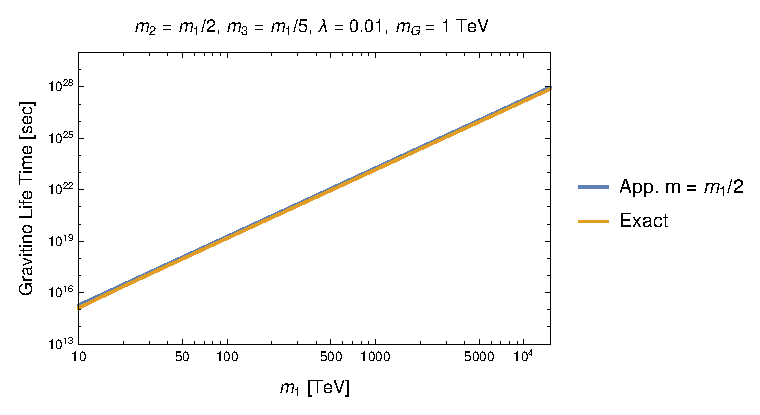
\includegraphics[scale=0.8]{GravitinoDecaym1m2m3Final}
\par\end{centering}

\caption{\label{fig:Gravitino-life-time}Gravitino life time in Trilinear RpV
for $\lambda_{ijk}=0.01,\,m_{G}=1\,\mbox{TeV}$. For simplicity we
use $m_{1},\,m_{2},\,m_{3}$ and $m$ instead of $m_{\tilde{\nu}_{iL}},\,m_{\tilde{e}_{jL}},\,m_{\tilde{e}_{kR}}$
and $\tilde{m}$.}
\end{figure}


Therefore, we can confidently derive the following expression for
the gravitino lifetime,

\begin{equation}
\tau_{G}\approx7\times10^{28}\,\mbox{sec}\,\left(\frac{1}{\lambda_{ijk}\lambda_{ijk}}\right)\left(\frac{\tilde{m}}{10^{8}\mbox{\,GeV}}\right)^{4}\left(\frac{1\,\mbox{TeV}}{m_{G}}\right)^{7}\label{eq:GravLifeTime}
\end{equation}


\noindent where we have normalized with respect to $10^{28}\mbox{ sec}$
since this is the order of magnitude required by experiments such
as AMS-02 and Fermi-LAT in order to fit the electron positron data
in the first case or to avoid gamma ray constraints in the second.


\section{Neutrino Masses}

In trilinear RpV the neutrino mass matrix receives contributions from
1-loop diagrams that contain both a charged lepton and the corresponding
slepton. Indeed, we have derived the following (preliminary) expression

\begin{eqnarray*}
M_{ij}^{\nu\,(1)} & \approx & \frac{1}{16\pi^{2}}\sum_{gr}s_{\tilde{l}}c_{\tilde{l}}(\lambda_{igr}\lambda_{jrg}+\lambda_{jgr}\lambda_{irg})m_{g}\ln\frac{m_{\tilde{l}_{r2}}^{2}}{m_{\tilde{l}_{r1}}^{2}}
\end{eqnarray*}


\noindent where $i$ and $j$ are neutrino generation indices that
run from 1 to 3. $g$ is a charged lepton index that also run from
1 to 3, as well as $r$ which is a slepton index. Thus, it can be
seen that for order one $s_{\tilde{l}}$, $c_{\tilde{l}}$ and $\ln(m_{l_{r2}}^{2}/m_{l_{r1}}^{2})$
we can get neutrino masses around the eV scale for $\lambda_{ijk}\approx0.01$
even for $m_{g}\approx m_{e}$. 

Indeed, by following the expressions given in hep-ph/0410242 for the
contribution of $\lambda'$ trilinear terms, we can get by analogy
that the dominant term in the leptonic sector is 

\begin{eqnarray*}
M_{ij}^{\nu\,(1)} & \approx & \frac{1}{8\pi^{2}}\lambda_{i23}\lambda_{j32}\frac{m_{\mu}m_{\tau}A_{\tau}}{\tilde{m}^{2}}\\
 & \approx & 2\times10^{-2}\mbox{eV}\,\lambda_{i23}\lambda_{j32}\,\left(\frac{10^{8}\mbox{\,GeV}}{\tilde{m}}\right)\\
 & \approx & 2\times10^{-2}\mbox{eV}\,(\lambda_{i23}\lambda_{j32})^{5/4}\left(\frac{\tau_{G}}{7\times10^{\text{28}}\,\mbox{sec}}\right)^{1/4}\left(\frac{m_{G}}{1\,\mbox{TeV}}\right)^{7/4}
\end{eqnarray*}


\noindent where $A_{\tau}$ is a free parameter that can be considered
of order $\tilde{m}$, as it is done in hep-ph/0410242. Thus, if we
consider this formula together with Eq. \ref{eq:GravLifeTime} we
see that we can have contributions to the neutrino mass matrix of
order $10^{-2}\mbox{eV}$ for trilinear couplings and a scalar mass
which are compatible with $\tau_{G}\approx10^{28}\mbox{ sec}$.
\end{document}
